% Options for packages loaded elsewhere
\PassOptionsToPackage{unicode}{hyperref}
\PassOptionsToPackage{hyphens}{url}
\PassOptionsToPackage{dvipsnames,svgnames,x11names}{xcolor}
%
\documentclass[
  12pt,
  letterpaper,
]{article}

\usepackage{amsmath,amssymb}
\usepackage{iftex}
\ifPDFTeX
  \usepackage[T1]{fontenc}
  \usepackage[utf8]{inputenc}
  \usepackage{textcomp} % provide euro and other symbols
\else % if luatex or xetex
  \usepackage{unicode-math}
  \defaultfontfeatures{Scale=MatchLowercase}
  \defaultfontfeatures[\rmfamily]{Ligatures=TeX,Scale=1}
\fi
\usepackage{lmodern}
\ifPDFTeX\else  
    % xetex/luatex font selection
    \setmainfont[]{Libertinus-serif}
    \setsansfont[]{Jost}
  \setmathfont[]{Libertinus-math}
\fi
% Use upquote if available, for straight quotes in verbatim environments
\IfFileExists{upquote.sty}{\usepackage{upquote}}{}
\IfFileExists{microtype.sty}{% use microtype if available
  \usepackage[]{microtype}
  \UseMicrotypeSet[protrusion]{basicmath} % disable protrusion for tt fonts
}{}
\makeatletter
\@ifundefined{KOMAClassName}{% if non-KOMA class
  \IfFileExists{parskip.sty}{%
    \usepackage{parskip}
  }{% else
    \setlength{\parindent}{0pt}
    \setlength{\parskip}{6pt plus 2pt minus 1pt}}
}{% if KOMA class
  \KOMAoptions{parskip=half}}
\makeatother
\usepackage{xcolor}
\usepackage[margin=1in]{geometry}
\setlength{\emergencystretch}{3em} % prevent overfull lines
\setcounter{secnumdepth}{-\maxdimen} % remove section numbering


\providecommand{\tightlist}{%
  \setlength{\itemsep}{0pt}\setlength{\parskip}{0pt}}\usepackage{longtable,booktabs,array}
\usepackage{calc} % for calculating minipage widths
% Correct order of tables after \paragraph or \subparagraph
\usepackage{etoolbox}
\makeatletter
\patchcmd\longtable{\par}{\if@noskipsec\mbox{}\fi\par}{}{}
\makeatother
% Allow footnotes in longtable head/foot
\IfFileExists{footnotehyper.sty}{\usepackage{footnotehyper}}{\usepackage{footnote}}
\makesavenoteenv{longtable}
\usepackage{graphicx}
\makeatletter
\def\maxwidth{\ifdim\Gin@nat@width>\linewidth\linewidth\else\Gin@nat@width\fi}
\def\maxheight{\ifdim\Gin@nat@height>\textheight\textheight\else\Gin@nat@height\fi}
\makeatother
% Scale images if necessary, so that they will not overflow the page
% margins by default, and it is still possible to overwrite the defaults
% using explicit options in \includegraphics[width, height, ...]{}
\setkeys{Gin}{width=\maxwidth,height=\maxheight,keepaspectratio}
% Set default figure placement to htbp
\makeatletter
\def\fps@figure{htbp}
\makeatother
% definitions for citeproc citations
\NewDocumentCommand\citeproctext{}{}
\NewDocumentCommand\citeproc{mm}{%
  \begingroup\def\citeproctext{#2}\cite{#1}\endgroup}
\makeatletter
 % allow citations to break across lines
 \let\@cite@ofmt\@firstofone
 % avoid brackets around text for \cite:
 \def\@biblabel#1{}
 \def\@cite#1#2{{#1\if@tempswa , #2\fi}}
\makeatother
\newlength{\cslhangindent}
\setlength{\cslhangindent}{1.5em}
\newlength{\csllabelwidth}
\setlength{\csllabelwidth}{3em}
\newenvironment{CSLReferences}[2] % #1 hanging-indent, #2 entry-spacing
 {\begin{list}{}{%
  \setlength{\itemindent}{0pt}
  \setlength{\leftmargin}{0pt}
  \setlength{\parsep}{0pt}
  % turn on hanging indent if param 1 is 1
  \ifodd #1
   \setlength{\leftmargin}{\cslhangindent}
   \setlength{\itemindent}{-1\cslhangindent}
  \fi
  % set entry spacing
  \setlength{\itemsep}{#2\baselineskip}}}
 {\end{list}}
\usepackage{calc}
\newcommand{\CSLBlock}[1]{\hfill\break\parbox[t]{\linewidth}{\strut\ignorespaces#1\strut}}
\newcommand{\CSLLeftMargin}[1]{\parbox[t]{\csllabelwidth}{\strut#1\strut}}
\newcommand{\CSLRightInline}[1]{\parbox[t]{\linewidth - \csllabelwidth}{\strut#1\strut}}
\newcommand{\CSLIndent}[1]{\hspace{\cslhangindent}#1}

% -----------------------
% CUSTOM PREAMBLE STUFF
% -----------------------

% -----------------
% Title block stuff
% -----------------

% Abstract
\usepackage[runin]{abstract}
\renewcommand{\abstractnamefont}{\sffamily\small\bfseries}
\renewcommand{\abstracttextfont}{\sffamily\small}
\setlength{\absleftindent}{5pt}
\setlength{\absrightindent}{\absleftindent}

% Title
\usepackage{titling}
\pretitle{\par\begin{flushleft}\LARGE\sffamily\bfseries}
\posttitle{\par\end{flushleft}\vskip 10pt}

% Keywords
\newenvironment{keywords}
{\small\sffamily{\sffamily\small\bfseries{Keywords.}}}

% Authors
\usepackage{orcidlink}  % Create automatic ORCID icons/links
%\renewcommand{\and}{\end{tabular} \hskip 3em \begin{tabular}[t]{@{\hspace{0em}}l@{}}}
\preauthor{\begin{flushleft}
           \lineskip 1.5em}
\postauthor{\end{flushleft}}

% ------------------
% Section headings
% ------------------
\usepackage{titlesec}
\titleformat*{\section}{\Large\sffamily\bfseries\raggedright}
\titleformat*{\subsection}{\large\sffamily\bfseries\raggedright}
\titleformat*{\subsubsection}{\normalsize\sffamily\bfseries\raggedright}
\titleformat*{\paragraph}{\small\sffamily\bfseries\raggedright}

%\titlespacing{<command>}{<left>}{<before-sep>}{<after-sep>}
% Starred version removes indentation in following paragraph
\titlespacing*{\section}{0em}{2em}{0.1em}
\titlespacing*{\subsection}{0em}{1.25em}{0.1em}
\titlespacing*{\subsubsection}{0em}{0.75em}{0em}

% ------------------
% Headers/Footers
% ------------------
\usepackage{fancyhdr}
\pagestyle{fancy}
\fancyhf{}
\fancyhead[L,C,R]{}
\fancyfoot[L,C]{}
\fancyfoot[R]{\thepage}
\renewcommand{\headrulewidth}{1pt}
\fancypagestyle{plain}{%
    \renewcommand{\headrulewidth}{0pt}%
    \fancyhf{}%
    \fancyfoot[R]{\thepage}%
}
\renewcommand\footnoterule{\rule{\linewidth}{0.1pt}\vspace{5pt}}

% ------------------
% Captions
% ------------------
\usepackage[labelfont=bf,labelsep=period]{caption}
\captionsetup[figure]{font=footnotesize,justification=raggedright,singlelinecheck=false,format=hang}


% ---------------------------
% END CUSTOM PREAMBLE STUFF
% ---------------------------
\usepackage{float}
\usepackage{tabularray}
\usepackage[normalem]{ulem}
\usepackage{graphicx}
\usepackage{rotating}
\UseTblrLibrary{booktabs}
\UseTblrLibrary{siunitx}
\NewTableCommand{\tinytableDefineColor}[3]{\definecolor{#1}{#2}{#3}}
\newcommand{\tinytableTabularrayUnderline}[1]{\underline{#1}}
\newcommand{\tinytableTabularrayStrikeout}[1]{\sout{#1}}
#import "@preview/mitex:0.2.4": *
\makeatletter
\@ifpackageloaded{caption}{}{\usepackage{caption}}
\AtBeginDocument{%
\ifdefined\contentsname
  \renewcommand*\contentsname{Tabla de contenidos}
\else
  \newcommand\contentsname{Tabla de contenidos}
\fi
\ifdefined\listfigurename
  \renewcommand*\listfigurename{Listado de Figuras}
\else
  \newcommand\listfigurename{Listado de Figuras}
\fi
\ifdefined\listtablename
  \renewcommand*\listtablename{Listado de Tablas}
\else
  \newcommand\listtablename{Listado de Tablas}
\fi
\ifdefined\figurename
  \renewcommand*\figurename{Figura}
\else
  \newcommand\figurename{Figura}
\fi
\ifdefined\tablename
  \renewcommand*\tablename{Tabla}
\else
  \newcommand\tablename{Tabla}
\fi
}
\@ifpackageloaded{float}{}{\usepackage{float}}
\floatstyle{ruled}
\@ifundefined{c@chapter}{\newfloat{codelisting}{h}{lop}}{\newfloat{codelisting}{h}{lop}[chapter]}
\floatname{codelisting}{Listado}
\newcommand*\listoflistings{\listof{codelisting}{Listado de Listados}}
\makeatother
\makeatletter
\makeatother
\makeatletter
\@ifpackageloaded{caption}{}{\usepackage{caption}}
\@ifpackageloaded{subcaption}{}{\usepackage{subcaption}}
\makeatother

\ifLuaTeX
\usepackage[bidi=basic]{babel}
\else
\usepackage[bidi=default]{babel}
\fi
\babelprovide[main,import]{spanish}
\ifPDFTeX
\else
\babelfont{rm}[]{Libertinus-serif}
\fi
% get rid of language-specific shorthands (see #6817):
\let\LanguageShortHands\languageshorthands
\def\languageshorthands#1{}
\ifLuaTeX
  \usepackage{selnolig}  % disable illegal ligatures
\fi
\usepackage{bookmark}

\IfFileExists{xurl.sty}{\usepackage{xurl}}{} % add URL line breaks if available
\urlstyle{same} % disable monospaced font for URLs
\hypersetup{
  pdftitle={La Mejor Masa de Pizza para Marcelo},
  pdfauthor={Miguel Equihua},
  pdflang={es},
  pdfkeywords={Quarto, Typst, format},
  colorlinks=true,
  linkcolor={blue},
  filecolor={Maroon},
  citecolor={Blue},
  urlcolor={red},
  pdfcreator={LaTeX via pandoc}}



\title{La Mejor Masa de Pizza para Marcelo\thanks{This template is
inspired by Kieran Healy's
\href{https://github.com/kjhealy/latex-custom-kjh}{LaTeX and Rmd
template} and Andrew Heiss's
\href{https://github.com/andrewheiss/hikmah-academic-quarto}{Hikmah
Quarto template}.}}
% subtitles do not seem to work with article class?
%%\usepackage{etoolbox}
%\makeatletter
%\providecommand{\subtitle}[1]{% add subtitle to \maketitle
%  \apptocmd{\@title}{\par {\large #1 \par}}{}{}
%}
%\makeatother
%%\subtitle{Uso de Quarto + Typst para reportes científicos}

\author{
{\bfseries \normalsize Miguel Equihua~\orcidlink{0000-0001-5306-7397}}%
 \\%
 \small Inecol,  \\%
{\footnotesize \url{miguel.equihua@inecol.mx}} \\\vspace{10pt}
}

\predate{}
\postdate{}
\date{}
\begin{document}

% for some reason this does not work in header
\renewcommand{\abstractname}{Abstract.}

% add the short title to the fancy header

\maketitle
%\noindent \rule{\linewidth}{.5pt}
\begin{abstract}
Duis ornare ex ac iaculis pretium. Maecenas sagittis odio id erat
pharetra, sit amet consectetur quam sollicitudin. Vivamus pharetra quam
purus, nec sagittis risus pretium at. Nullam feugiat, turpis ac accumsan
interdum, sem tellus blandit neque, id vulputate diam quam semper nisl.
Donec sit amet enim at neque porttitor aliquet. Phasellus facilisis
nulla eget placerat eleifend. Vestibulum non egestas eros, eget lobortis
ipsum. Nulla rutrum massa eget enim aliquam, id porttitor erat luctus.
Nunc sagittis quis eros eu sagittis. Pellentesque dictum, erat at
pellentesque sollicitudin, justo augue pulvinar metus, quis rutrum est
mi nec felis. Vestibulum efficitur mi lorem, at elementum purus
tincidunt a. Aliquam finibus enim magna, vitae pellentesque erat
faucibus at. Nulla mauris tellus, imperdiet id lobortis et, dignissim
condimentum ipsum. Morbi nulla orci, varius at aliquet sed, facilisis id
tortor. Donec ut urna nisi.
\end{abstract}
\begin{keywords}
\def\sep{;\ }
Quarto\sep Typst\sep 
format
\end{keywords}
%\noindent \rule{\linewidth}{.5pt}


This document shows a practical usage of the template.

I use the Palmer penguins dataset (Horst, Hill, y Gorman 2020) to
demonstrate the features of the template. The code is available
\href{https://github.com/kazuyanagimoto/quarto-academic-typst}{here}.

\section{Section as Heading Level 1}\label{section-as-heading-level-1}

Section numbering can be specified in the YAML
\texttt{section-numbering} field as other Typst templates.

\subsection{Subsection as Heading Level
2}\label{subsection-as-heading-level-2}

You can use LaTeX math expressions:

\[
Y_{it} = \alpha_i + \lambda_t + \sum_{k \neq -1} \tau_h \mathbb{1}\{E_i + k = t\} +
\varepsilon_{it}.
\]

I choose a mathematical font which supports the indicator function
\(\mathbb{1}\{\cdot\}\). Currently, I use the Libertinus-math font.

\subsubsection{Subsubsection as Heading Level
3}\label{subsubsection-as-heading-level-3}

I don't use and don't recommend using heading levels 3 and below but it
works.

\subsection{Citation}\label{citation}

You can cite a reference like this (Katsushika 1831) or Horst, Hill, y
Gorman (2020). Typst has some built-in citation styles. Check the
\href{https://typst.app/docs/reference/model/bibliography/\#parameters-style}{Typst
documentation} for more information.

\section{Figures and Tables}\label{figures-and-tables}

\subsection{Figures}\label{figures}

As Figura~\ref{fig-facet} shows, the caption is displayed below the
figure. As a caption of the figure (\texttt{fig-cap}), I use bold text
for the title and use a normal text for the description.

\begin{figure}[!t]

\centering{

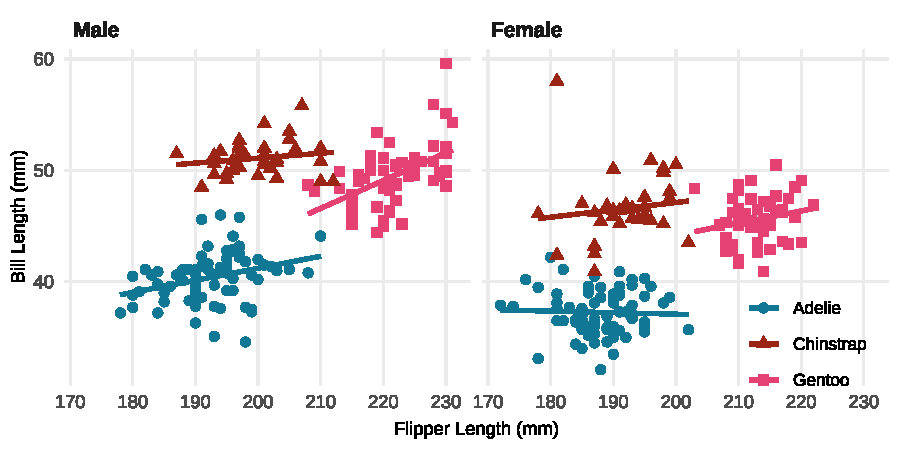
\includegraphics{articulo-pizza_files/figure-pdf/fig-facet-1.pdf}

}

\caption{\label{fig-facet}\textbf{Flipper Length and Bill Length of
Penguins}. The x-axis shows the flipper length, and the y-axis shows the
bill length.}

\end{figure}%

When I want to show multiple figures side by side, I use the
\texttt{patchwork} package. The reason why I don't use the
\texttt{layout-col} option is that the caption is also split into two
parts.

\begin{figure}[!t]

\centering{

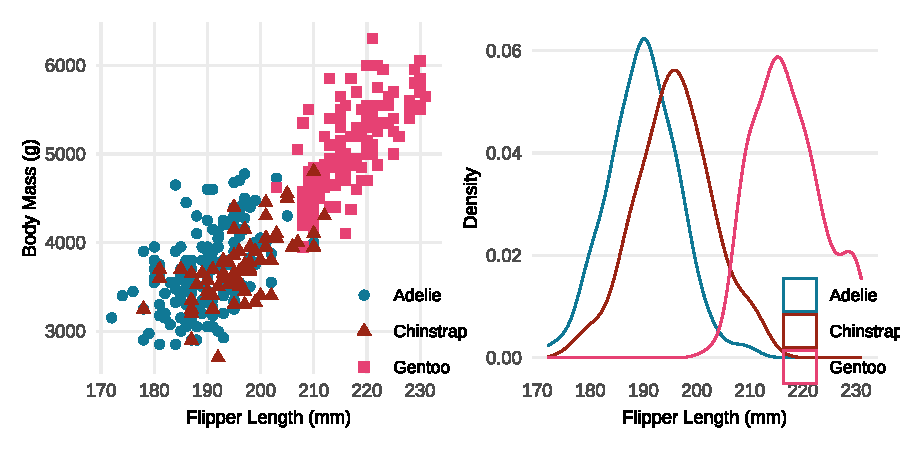
\includegraphics{articulo-pizza_files/figure-pdf/fig-patchwork-1.pdf}

}

\caption{\label{fig-patchwork}\textbf{Characteristics of Penguins}. The
left panel shows the relationship between flipper length and body mass.
The right panel shows the density of flipper length.}

\end{figure}%

\subsection{Tables}\label{tables}

You can use
\href{https://vincentarelbundock.github.io/tinytable/}{tinytable} for
general tables and
\href{https://vincentarelbundock.github.io/modelsummary/}{modelsummary}
for regression tables. As Tabla~\ref{tbl-sum-penguins} shows, the
caption is displayed above the table. The notes of the table can be
added using the \texttt{notes} argument of the \texttt{tinytable::tt()}
function.

\begin{table}

\caption{\label{tbl-sum-penguins}Summary Statistics of Penguins}

\centering{

\centering
\begin{talltblr}[         %% tabularray outer open
entry=none,label=none,
note{}={_Notes_: Data from Palmer penguins dataset.},
]                     %% tabularray outer close
{                     %% tabularray inner open
colspec={Q[]Q[]Q[]Q[]Q[]Q[]Q[]Q[]Q[]},
cell{1}{2}={c=4,}{halign=c,},
cell{1}{6}={c=4,}{halign=c,},
}                     %% tabularray inner close
\toprule
& Male &  &  &  & Female &  &  &  \\ \cmidrule[lr]{2-5}\cmidrule[lr]{6-9}
& Bill Length (mm) & Bill Depth (mm) & Flipper Length (mm) & Body Mass (g) & Bill Length (mm) & Bill Depth (mm) & Flipper Length (mm) & Body Mass (g) \\ \midrule %% TinyTableHeader
Adelie & 40.39 & 19.07 & 192.4 & 4043 & 37.26 & 17.62 & 187.8 & 3369 \\
Gentoo & 49.47 & 15.72 & 221.5 & 5485 & 45.56 & 14.24 & 212.7 & 4680 \\
Chinstrap & 51.09 & 19.25 & 199.9 & 3939 & 46.57 & 17.59 & 191.7 & 3527 \\
\bottomrule
\end{talltblr}

}

\end{table}%

Since the default backend of \texttt{modelsummary} is
\texttt{tinytable}, you can use the customization options of
\texttt{tinytable} for \texttt{modelsummary}. In
Tabla~\ref{tbl-regression}, I use \texttt{tinytable::group\_tt()}
function to group the regression results by the dependent variables

\begin{table}

\caption{\label{tbl-regression}Regression Results of Penguins}

\centering{

\centering
\begin{talltblr}[         %% tabularray outer open
entry=none,label=none,
note{}={+ p \num{< 0.1}, * p \num{< 0.05}, ** p \num{< 0.01}},
note{ }={\_Notes\_: Data from Palmer penguins dataset.},
]                     %% tabularray outer close
{                     %% tabularray inner open
colspec={Q[]Q[]Q[]Q[]Q[]Q[]Q[]},
column{3,4,6,7}={}{halign=c,},
column{1}={}{halign=l,},
cell{2}{2}={}{halign=c,},
cell{2}{5}={}{halign=c,},
cell{3}{2}={}{halign=c,},
cell{3}{5}={}{halign=c,},
cell{4}{2}={}{halign=c,},
cell{4}{5}={}{halign=c,},
cell{5}{2}={}{halign=c,},
cell{5}{5}={}{halign=c,},
cell{6}{2}={}{halign=c,},
cell{6}{5}={}{halign=c,},
cell{7}{2}={}{halign=c,},
cell{7}{5}={}{halign=c,},
cell{8}{2}={}{halign=c,},
cell{8}{5}={}{halign=c,},
cell{9}{2}={}{halign=c,},
cell{9}{5}={}{halign=c,},
cell{10}{2}={}{halign=c,},
cell{10}{5}={}{halign=c,},
cell{11}{2}={}{halign=c,},
cell{11}{5}={}{halign=c,},
cell{1}{2}={c=3,}{halign=c, halign=c,},
cell{1}{5}={c=3,}{halign=c, halign=c,},
hline{11}={1,2,3,4,5,6,7}{solid, black, 0.05em},
}                     %% tabularray inner close
\toprule
& Bill Length (mm) &  &  & Body Mass (g) &  &  \\ \cmidrule[lr]{2-4}\cmidrule[lr]{5-7}
& (1) & (2) & (3) & (4) & (5) & (6) \\ \midrule %% TinyTableHeader
Chinstrap & \num{10.042}** & \num{10.010}** & \num{10.037}** & \num{32.426} & \num{26.924} & \num{27.229} \\
& (\num{0.432}) & (\num{0.341}) & (\num{0.340}) & (\num{67.512}) & (\num{46.483}) & (\num{46.587}) \\
Gentoo & \num{8.713}** & \num{8.698}** & \num{8.693}** & \num{1375.354}** & \num{1377.858}** & \num{1377.813}** \\
& (\num{0.360}) & (\num{0.287}) & (\num{0.286}) & (\num{56.148}) & (\num{39.104}) & (\num{39.163}) \\
Male &  & \num{3.694}** & \num{3.694}** &  & \num{667.555}** & \num{667.560}** \\
&  & (\num{0.255}) & (\num{0.254}) &  & (\num{34.704}) & (\num{34.755}) \\
Year &  &  & \num{0.324}* &  &  & \num{3.629} \\
&  &  & (\num{0.156}) &  &  & (\num{21.428}) \\
Observations & \num{342} & \num{333} & \num{333} & \num{342} & \num{333} & \num{333} \\
\bottomrule
\end{talltblr}

}

\end{table}%

While \texttt{tinytable} generates compatible tables between LaTeX and
Typst, it does not support LaTeX math expressions for Typst tables. I
think the compatibility between LaTeX and Typst is crucial for academic
writing because it guarantees that the document can be easily converted
to LaTeX for submission to journals.

A workaround is to use
\href{https://typst.app/universe/package/mitex/}{MiTeX}, a Typst package
that allows you to use LaTeX math expressions in Typst. I write a custom
theme for \texttt{tinytable} to convert LaTeX math expressions to MiTeX
expressions. The following table includes LaTeX math expressions but
will be converted to MiTeX expressions in the Typst output.

\begin{table}

\caption{\label{tbl-math}Math Symbols}

\centering{

\centering
\begin{tblr}[         %% tabularray outer open
]                     %% tabularray outer close
{                     %% tabularray inner open
colspec={Q[]},
}                     %% tabularray inner close
\toprule
Math \\ \midrule %% TinyTableHeader
$\alpha$ \\
$a_{it}$ \\
$e^{i\pi} + 1 = 0$ \\
\bottomrule
\end{tblr}

}

\end{table}%

\section{Last words}\label{last-words}

I made this template for my working papers, so it may not be suitable
for other fields than economics. I am happy to receive feedback and
suggestions for improvement.



\section{Supplemental Figures}\label{supplemental-figures}

The section numbering will be changed to ``A.1.1'' in the appendix. The
second section in the appendix will be ``B''. On the other hand, the
figure numbering will be reset to ``A.1'', ``A.2'' so that it is clear
that these figures are part of the appendix. The ``A'' stands for the
``Appendix'', not the section numbering.

\begin{figure}[!t]

\centering{

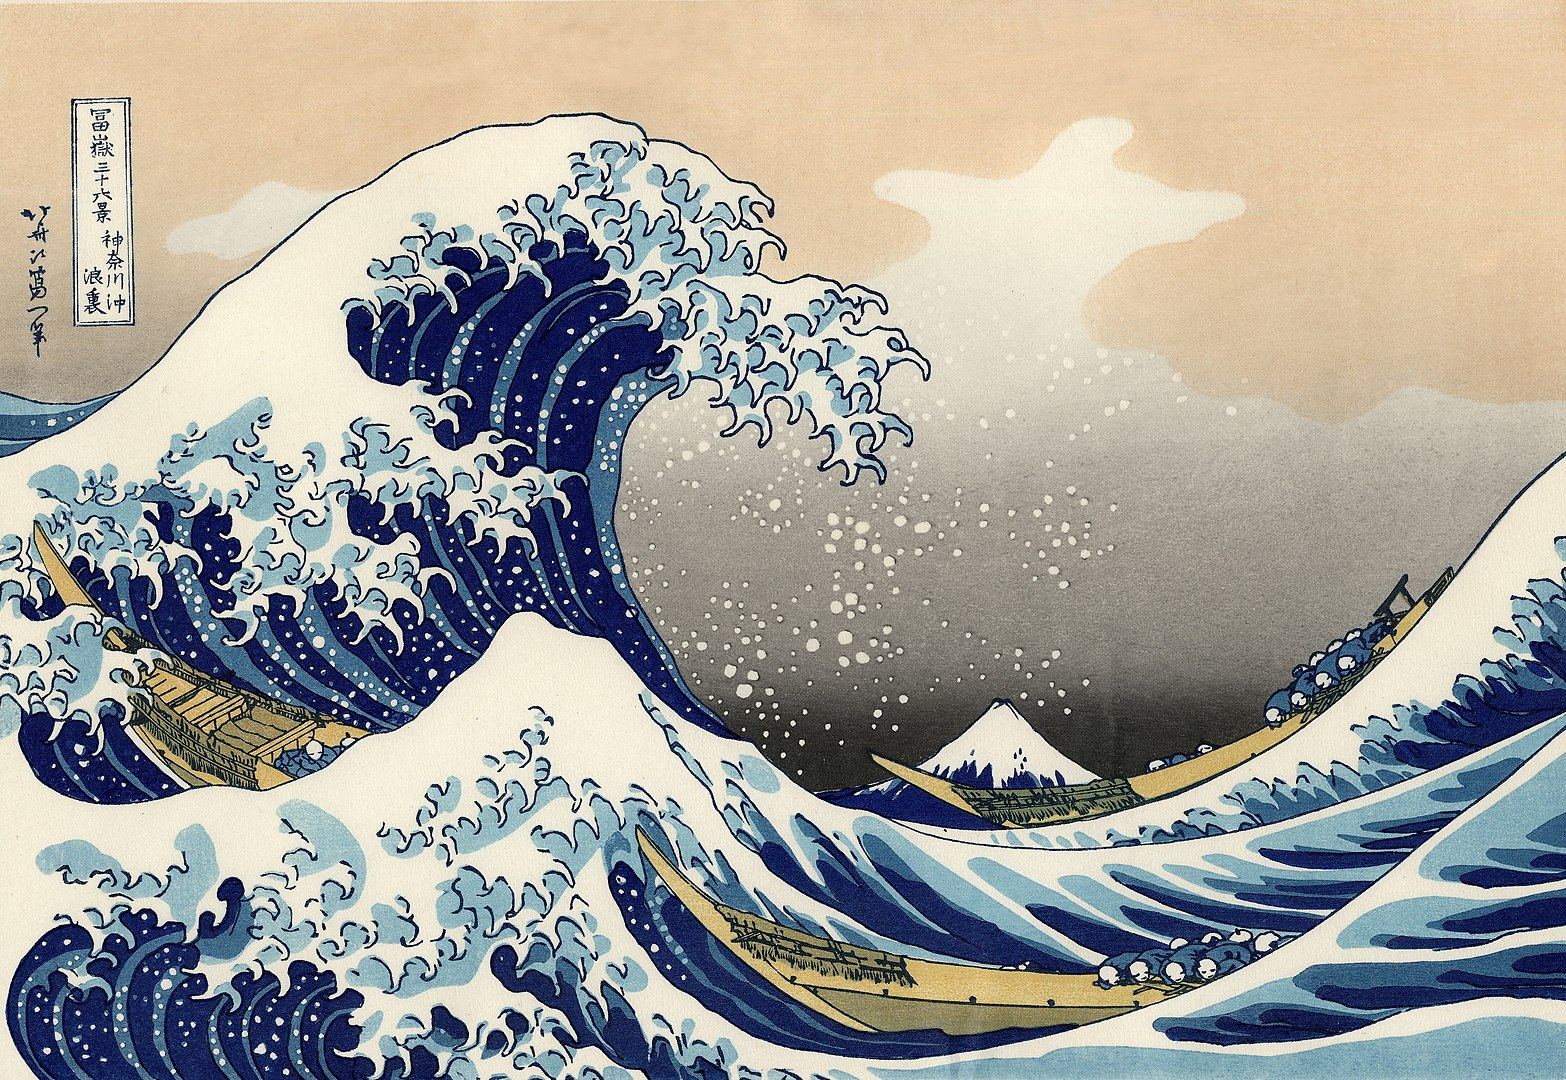
\includegraphics{img/hokusai_kanagawa.jpg}

}

\caption{\label{fig-img}\textbf{The Great Wave off Kanagawa}. A
woodblock print by Katsushika (1831).}

\end{figure}%

\newpage{}

\phantomsection\label{refs}
\begin{CSLReferences}{1}{0}
\bibitem[\citeproctext]{ref-horst2020}
Horst, Allison Marie, Alison Presmanes Hill, y Kristen B Gorman. 2020.
\emph{palmerpenguins: Palmer Archipelago (Antarctica) penguin data}.
\url{https://doi.org/10.5281/zenodo.3960218}.

\bibitem[\citeproctext]{ref-katsushika1831}
Katsushika, Hokusai. 1831. {«The Great Wave off Kanagawa»}.
\url{https://upload.wikimedia.org/wikipedia/commons/a/a5/Tsunami_by_hokusai_19th_century.jpg}.

\end{CSLReferences}




\end{document}
